\documentclass{anschreiben}

\usepackage{wrapfig}

\renewcommand{\deinName}{Ingo Blechschmidt und Rolf Wittmann}
\renewcommand{\deineMailAdresse}{iblech@speicherleck.de und rkw95@web.de}


\renewcommand{\datum}{\today}
\renewcommand{\betreff}{Matheschülerzirkel der Universität Augsburg}

\begin{document}

\newcommand{\direuch}{}

\newread\quelle
\openin\quelle=teilnehmende.csv
\read\quelle to \zeile

\loop
\read\quelle to \zeile
\ifeof\quelle\global\morefalse\else

\bearbeitezeile

\ifganzeklasse Liebe Schülerinnen und Schüler,\else
\ifweiblich Liebe\else Lieber\fi{} \vorname,\fi

\renewcommand{\direuch}{\ifganzeklasse euch\else dir\fi}

nach dem ausführlichen Beweis aus dem letzten Korrespondenzbrief geht es dieses
Mal in eine ganz andere Richtung, nämlich um \emph{unlösbare Aufgaben}.

\begin{center}
\includegraphics[scale=0.7]{unsolvable}\end{center}

Diese Aufgaben stellen wir aber nicht, weil wir besonders gemein sein wollen,
sondern weil auch unlösbare Probleme ein interessanter Bereich der Mathematik
sind. Wenn nämlich eine Mathematikerin auf solch eine unlösbare Aufgabe
stößt, dann möchte sie nicht einfach sagen: \emph{Ich kann diese Aufgabe nicht
lösen.} Sie möchte dann wenigstens sagen können: \emph{Ich kann diese Aufgabe nicht
lösen -- aber auch niemand anders wird diese Aufgabe jemals lösen können!} Und
in diesem Brief lernst du, wie auch du das sagen (und begründen!) kannst. Lass
dich wie immer nicht entmutigen, falls du mal eine Aufgabe nicht lösen kannst.

Es ist nicht weiter schlimm, eine Aufgabe auszulassen. Die Aufgaben bauen nicht
aufeinander auf, lassen sich aber zum Teil mit ähnlichen Ideen lösen. In der
Mathematik ist nicht nur das Ergebnis wichtig, sondern es gilt viel mehr der
Leitsatz: \emph{Der Weg ist das Ziel!} Denn nur wenn du alle deine Gedankengänge
aufschreibst, können wir dir eine angemessene Rückmeldung geben und dir genau
sagen, wo bei der Aufgabe der Haken war.

Wir haben noch drei besondere Ankündigungen für euch.

\begin{itemize}
\item Das Mathecamp 2018 findet vom 18. bis 26. August statt. Wie immer zieht
es uns nach Violau, wo wir vormittags in kleinen Gruppen Mathematik und
nachmittags je nach Wahl entweder noch mehr Mathematik, nerdige Freizeit
(Zauberwürfel, Programmieren, Basteln, Drohnen steuern und verlieren) oder
nicht in klassischer Hinsicht nerdige Freizeit (Sport, Musik) genießen möchten.
Die Anmeldung wird in etwa einer Woche freigeschaltet. Details:
\url{https://www.math.uni-augsburg.de/schueler/mathezirkel/}

\item Kurz vor Weihnachten gab es bei uns am Institut eine mathematische
Weihnachtsvorlesung zum Thema \emph{Die wundersame Welt der vierdimensionalen
Geometrie}. Die Aufzeichnung ist online, vielleicht interessiert sie euch:
\url{https://www.youtube.com/watch?v=d19zmiVBLS8} Dabei seht ihr auch gleich,
wie es bei uns in Hörsälen manchmal so zu geht. Fragen zum Thema sind sehr
willkommen!

\item Wir haben noch einen anderen Zirkelbrief für dieses Mal vorbereitet, uns
in letzter Sekunde aber dann dagegen entschieden, ihn zu verschicken, weil nicht
alle von euch schon Differentialrechnung kennen. Wenn ihr wisst, dass die
Ableitung von~$x^2$ gleich~$2x$ ist, dann schreibt uns schnell eine einzeilige
Mail. Dann schicken wir euch diesen anderen Brief auch noch zu, wenn ihr
möchtet auch per Mail. In dem Brief geht es um mathematische
Alternativuniversen und um Zahlen, die so klein sind, dass ihr Quadrat Null
ist.
\end{itemize}

Beim nächsten Mal möchten wir die \emph{Grahamsche Zahl} vorstellen. Das ist
eine Zahl, die jede sinnvolle Größenvorstellung völlig sprengt. Sie ist so
groß, dass selbst bei winzigster Schrift das physische Universum zu klein ist,
um sie jemals vollständig niederzuschreiben. Und sogar die Anzahl der Stellen
dieser Zahl ist unaufschreibbar; und auch die Anzahl der Stellen \emph{dieser}
Zahl, und noch oft so weiter (wie oft, lässt sich nicht aufschreiben).
Illustrerweise lässt sich die letzte Ziffer dieser Zahl trotzdem berechnen, und
wir werden euch erklären, wie das geht.

Viele Grüße

Ingo und Rolf

\bigskip
\bigskip

PS: In etwa einem Monat wird ein Sonnenlicht reflektierender Satellit mit dem
bloßen Auge zu sehen sein. Auf \url{https://thehumanitystar.com/} könnt ihr
erfahren, wann genau das bei euch zu Hause sein wird!

\begin{center}
  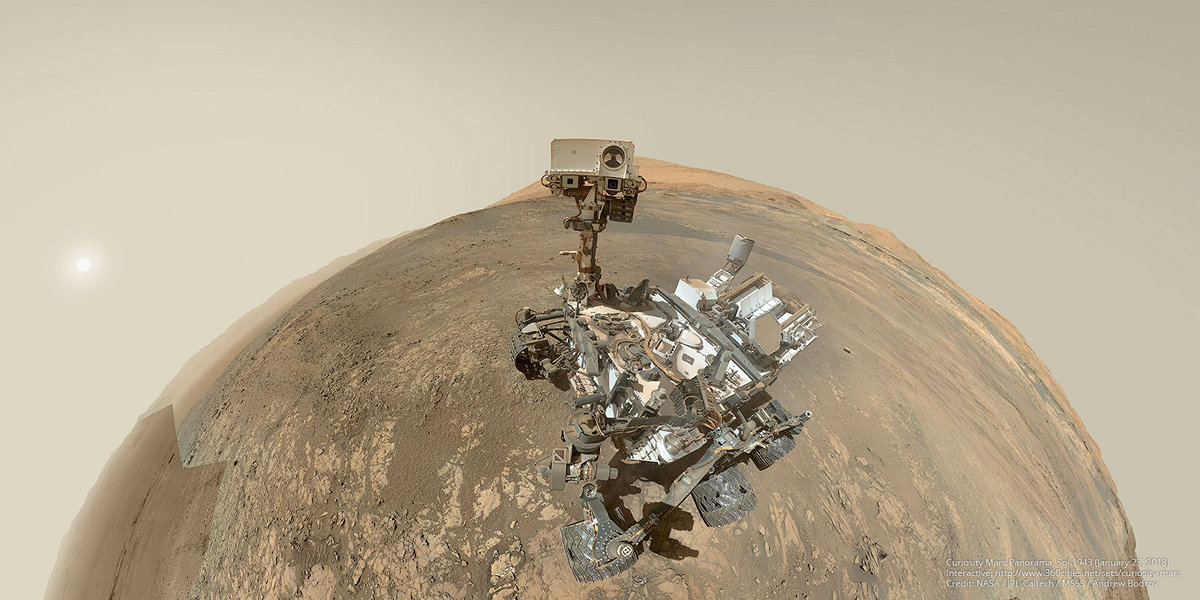
\includegraphics[width=0.8\textwidth]{selfie}

  Ein Selfie von Curiosity.

  Dieses Weltallfoto und andere (mit Erklärung!) gibt's unter:
  \url{https://apod.nasa.gov/apod/ap180126.html}
\end{center}

\newpage
\fi\ifmore\repeat

\closein\quelle

\end{document}
